%=================================================================
\section{Introduction}\label{sec-intro}


%\todo{Narrow down to a topic; Dig a hole; Fill the hole}
% \todo{Formula for Introduction}



%\gangli{``narrow in on topic'' reminds you 
%that readers and reviewers only know that this is a AI or HTM research paper (and maybe have read the title/abstract). 
%You need to help them figure out what topic and area of research paper this is. 
%You _don't_ need to wax poetic about the topic's importance.}

%\gangli{`dig a hole'' reminds you that 
%you need to convince the reader that there's a problem with the state of the world. 
%Prior work may exist but it's either missing something important or there's a missing opportunity. 
%The reader should be drooling for a bright future just out of reach.}

%\gangli{``fill the hole'' reminds you to show the reader 
%how and why the paper they're reading will fix these problems and deliver us into a better place. 
%You don't need a whirlwind summary of the technical details, 
%but you need readers convinced (and in a good mood) to keep reading.}

% \gangli{A good paper introduction is fairly formulaic. 
% If you follow a simple set of rules, 
% you can write a very good introduction. 
% The following outline can be varied. 
% For example, 
% you can use two paragraphs instead of one, 
% or you can place more emphasis on one aspect of the intro than another. 
% But in all cases, 
% all of the points below need to be covered in an introduction, 
% and in most papers, 
% you don't need to cover anything more in an introduction.}



%\todo{The importance of the area}
%\blindtext
% \todo{Motivation}
In a PUBG game, up to 100 players start in each match (matchId). Players can be on teams (groupId) which get ranked at the end of the game
(winPlacePerc) based on how many other teams are still alive when they
are eliminated. In game, players can pick up different munitions, revive
downed-but-not-out (knocked) teammates, drive vehicles, swim, run, shoot,
and experience all of the consequences – such as falling too far or running
themselves over and eliminating themselves. Different game behaviors will
lead to different final rankings, so the main purpose is to build a model to
predicts players’ finishing placement based on their final stats, on a scale
from 1 (first place) to 0 (last place).



%\todo{The problems faced by most current methods}
%\blindtext
% \todo{What is the specific problem considered in this paper?}
% This paragraph narrows down the topic area of the paper. 
% In the first paragraph you have established general context and importance. 
% Here you establish specific context and background.

%\todo{What can be addressed by existing methods; Why those problems are challenges to existing methods?}
%\blindtext
% \todo{Contribution}
In this paper, we show that how to use the different game actions to predict the final win places. It can 
help game player to get higher rank and help game data analyst to get higher correlation actions to help prefessional player
to get better win places in the competiton.
% This is the key paragraph in the intro - you summarize, 
% in one paragraph, 
% what are the main contributions of your paper given the context 
% you have established in paragraphs 1 and 2. 
% What is the general approach taken? 
% Why are the specific results significant? 
% This paragraph must be really good. 

% You should think about how to structure these one or 
% two paragraph summaries of what your paper is all about. 
% If there are two or three main results, 
% then you might consider itemizing them with bullets or in test. 
% \begin{itemize}
% 	\item e.g., First ...
% 	\item e.g., Second ...
% 	\item e.g., Third ...
% \end{itemize}
% If the results fall broadly into two categories, 
% you can bring out that distinction here. 
% For example, "Our results are both theoretical and applied in nature. 
% (two sentences follow, one each on theory and application)"

%\todo{What provides the motivation of this work? What are the research issues? What is the rationale of this work? }
%\blindtext
% \todo{At a high level what are the differences in what you are doing, and what others have done? }
% Keep this at a high level, 
% you can refer to a future section where specific details and differences will be given. 
% But it is important for the reader to know at a high level, 
% what is new about this work compared to other work in the area.

% %\todo{What we have done and what are the contributions.}
% %\blindtext
% \todo{A roadmap for the rest of the paper}
The remainder of this paper is structured as follows: 
In section 2, data visualizaiton will show the different game type proportion and relationship between two attributes.
In Section 3, use linear regression and decision tree to build model and predict.

% \gangli{A few general tips:
% Don't spend a lot of time into the introduction 
% telling the reader about what you don't do in the paper. 
% Be clear about what you do do.
% Does each paragraph have a theme sentence that sets the stage for the entire paragraph? Are the sentences and topics in the paragraph all related to each other?}

% \gangli{Does each paragraph have a theme 
% sentence that sets the stage for the entire paragraph? 
% Are the sentences and topics in the paragraph all related to each other?}

% \gangli{Do all of your tenses match up in a paragraph?}

% Test citation~\cite{BL12J01}. 
% \begin{JournalOnly}
% and~\citep{BJL11J01} or~\citet{BJL11J01}.
% \end{JournalOnly}

% This is for~\cref{tbl:overall-experiments}, 
% \todo[fancyline]{Testing.}
% and this is for~\cref{sec-conclusions}.
% \todo[noline]{A note with no line back to the text.}%
% \gangli{This is comment from Gang.}
% \qwu{Response from QW}

% Number:
% \num{123}.
% \numlist{10;30;50;70},
% \numrange{10}{30},
% \SIlist{10;30;45}{\metre},
% and
% \SI{10}{\percent}

% \missingfigure[figcolor=white]{Testing figcolor}


% \begin{ConferenceOnly}
% We have \SI{10}{\hertz},
% \si{\kilogram\metre\per\second},
% the range: \SIrange{10}{100}{\hertz}.
% $\nicefrac[]{1}{2}$.

% \missingfigure{Make a sketch of the structure of a trebuchet.}

% \end{ConferenceOnly}


% For~\cref{eq:test},
% as shown below:

% \begin{equation}\label{eq:test}
% a = b \times \sqrt{ab}
% \end{equation}

% \blindmathpaper

% \section{Data preprocess} \label{sec-preliminaries}

% \blindtext

% \gliMarker  %TODO: GLi Here


\section{Data visualizaiton} \label{sec-method}
\begin{itemize}
  \item Figure 1 shows the different game type proportion of all matched games.
  Most players choose to play squad fpp and duo fpp. So if players want to play with more players.
  \item Figure 2 shows long walking distance always means higher rank because if a player move a lot and survive,
  he always can get a higher rank. For players, if want to get higher win places, they need to keep moving.
\end{itemize}
\begin{figure}
  \centering
  % \selectcolormodel{rgb}
  % \missingfigure{Testing a long text string.}
  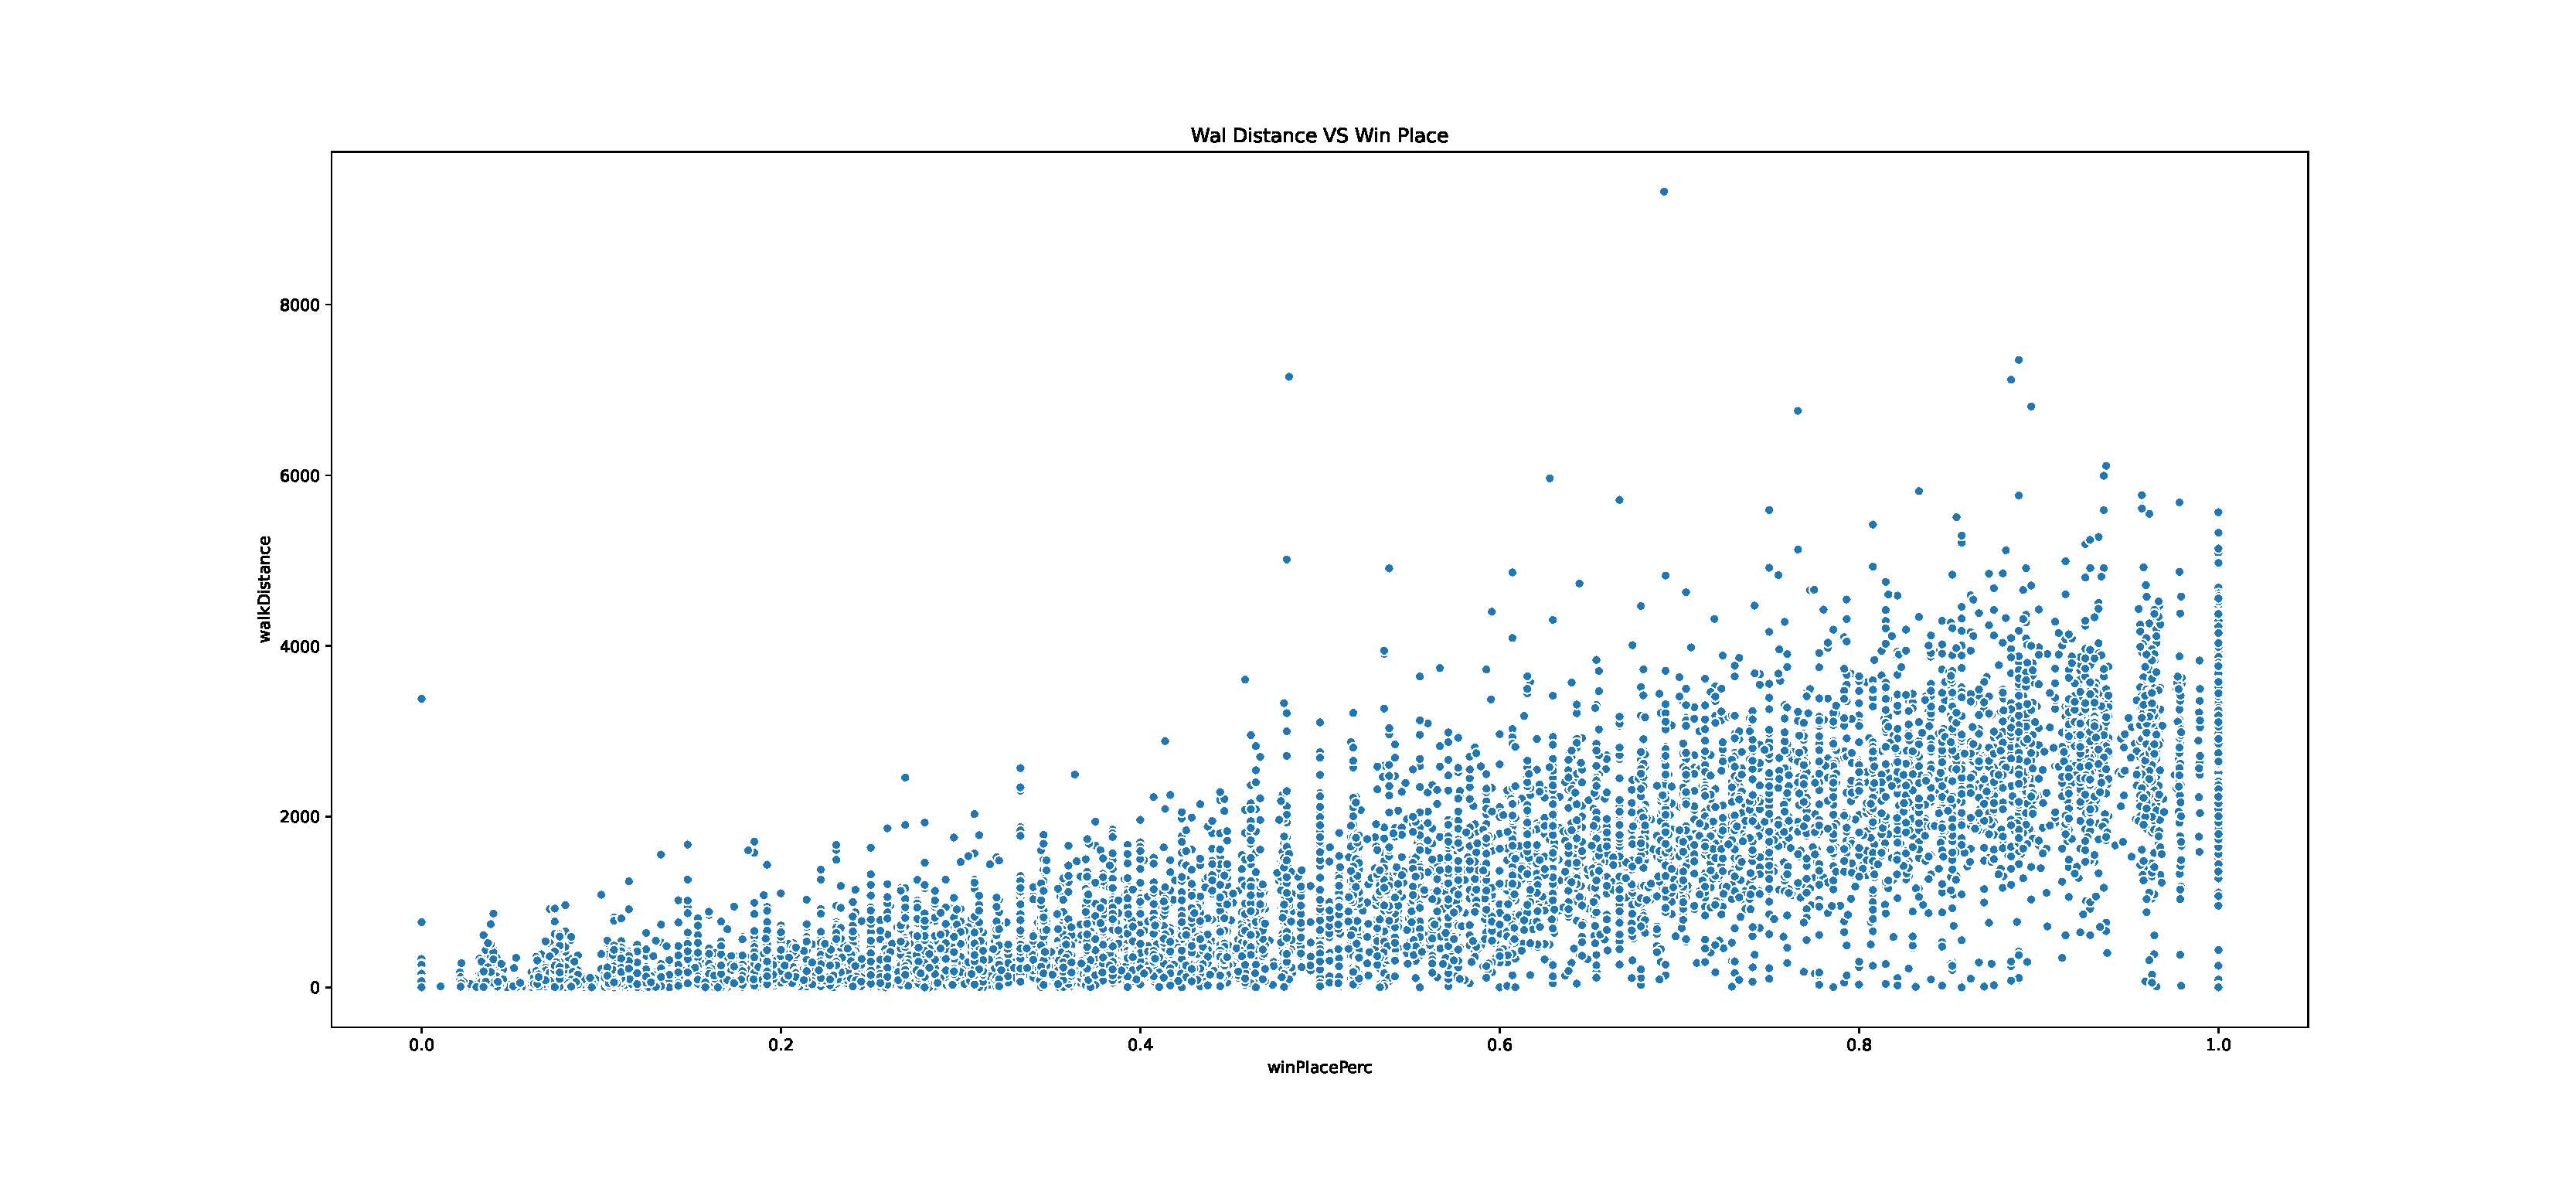
\includegraphics[width=1\textwidth]{scatter.eps}
  \caption{walking distance VS Win Place} 
  \label{scatter}
\end{figure}
\begin{figure}
  \centering
  % \selectcolormodel{rgb}
  % \missingfigure{Testing a long text string.}
  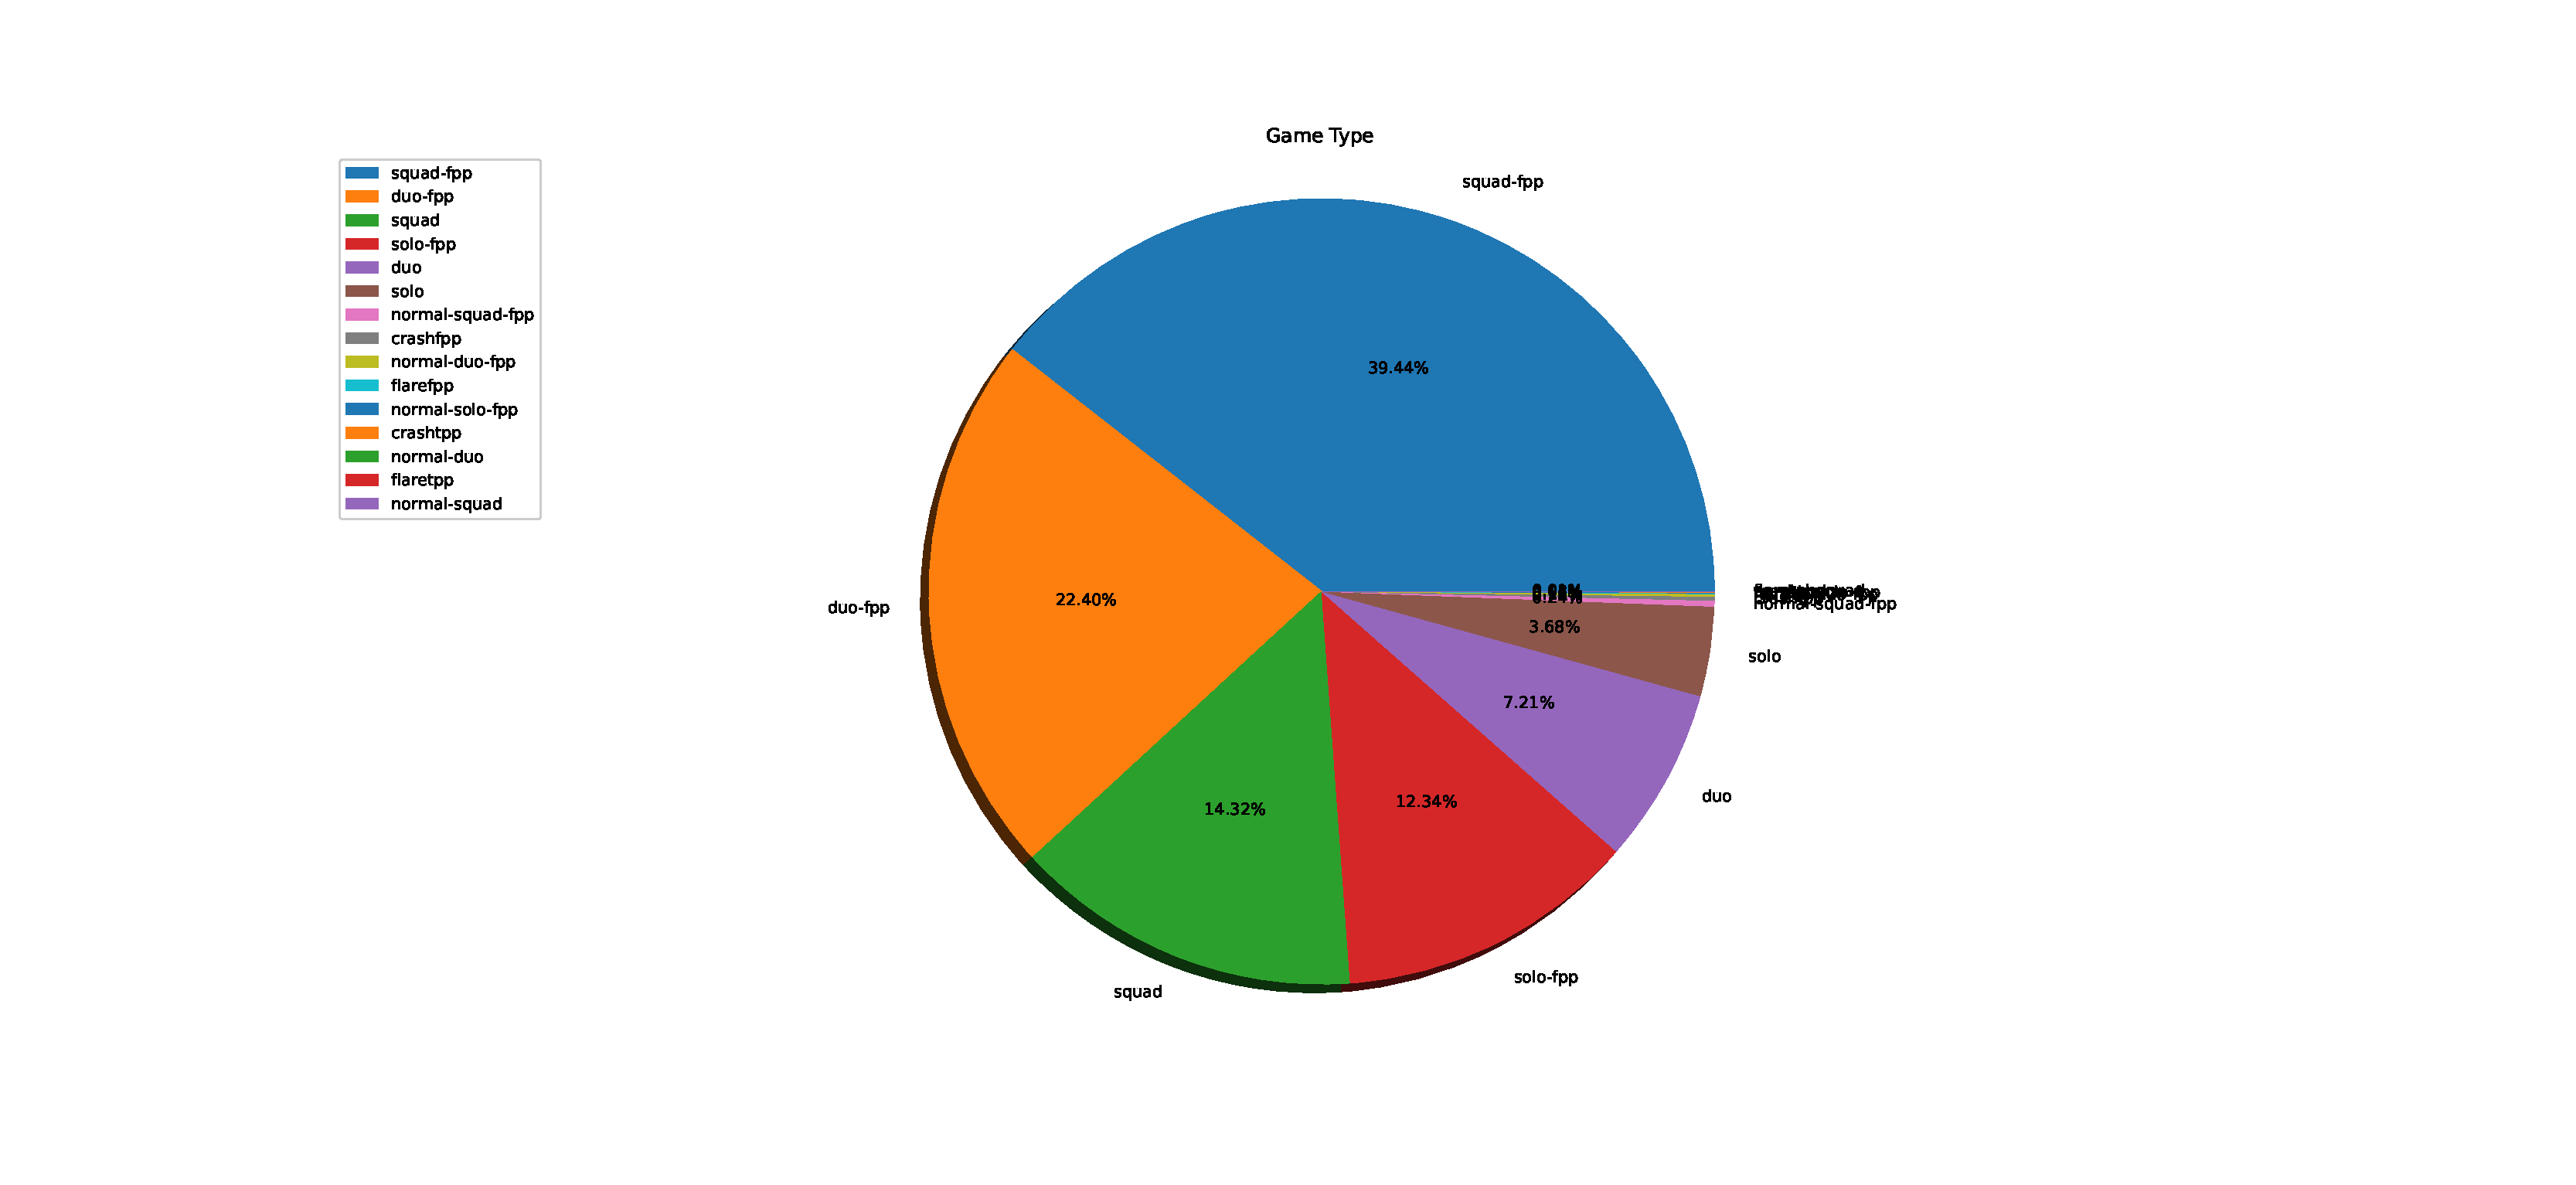
\includegraphics[width=1\textwidth]{pie.eps}
  \caption{game type proportion} 
  \label{pie}
\end{figure}
% \blindtext
% \blindlist{itemize}[3]
% \blinditemize
% \blindenumerate

% \blindmathtrue
% \blindmathfalse
% \blinddescription

% \qwuMarker %TODO: QWu Here

\section{Experiment and Analysis} \label{sec-experiment}
\begin{itemize}
  \item Base on table 1, we can see that linear regression model get lower MSE value, 
  it means that it has a higher accuracy and lower error value between predictions and actuals.
\end{itemize}

\begin{table}  \centering
  \caption{Precision Comparison}
  \label{tbl:overall-experiments}
  \begin{tabular}{cccc}
\toprule
    % after \\: \hline or \cline{col1-col2} \cline{col3-col4} ...
     & train MSE & test MSE \\
\midrule
    linear regression & 0.01564124116618947 & 0.015303007019988265
    \\
    decision tree & 0.01859312767771217 & 0.17048691321544765 \\
\bottomrule
\end{tabular}
\end{table}


\section{Conclusions} \label{sec-conclusions}
\begin{itemize}
  \item Both training and testing data shows that linear model get lower mean square error
  value.
  \item Most players choose to play squad-fpp and duo-fpp
  \item More walking distance always can bring higher win place.
\end{itemize}
% \blindtext

% \section*{Acknowledgement}

% \lipsum[1]


% The authors would like to thank \ldots

